\documentclass[12pt]{article}
\usepackage{booktabs}
\usepackage{graphicx}
\usepackage[margin=1.1in]{geometry}
\usepackage{float}
\restylefloat{table}

\setlength{\parskip}{1em}

\begin{document}
\begin{titlepage}
\begin{figure}[t]
    \centering
\includegraphics[width=0.15\textwidth]{logo}
\end{figure}
\begin{center}
    \textsc{ \LARGE{University of Sussex \\}}
	\textsc{School of Engineering and Informatics\\}
	\vspace{12mm}
	\fontsize{6mm}{7mm}\textnormal{Mathematics for Computing 2\\}
	\fontsize{10mm}{7mm}\selectfont
	\vspace{2mm}
    \textup{Assignment 1}\\
\end{center}

\vspace{25mm}

\centering{\large{Candidate number: 215800}}

\end{titlepage}
\tableofcontents

\clearpage

\section{Logic and Karnaugh maps}
\subsection{Truth table}

Here is the truth table.
\begin{table}[h]
\begin{tabular}{|l|l|l|l|l|l|l|l|l|l|l|}
\hline
A & B & C & D & Gate 1 & Gate 2 & Gate 3 & Gate 4 & Gate 5 & Gate 6 & OUT \\ \hline
0 & 0 & 0 & 0 & 1 & 0 & 0 & 0 & 1 & 0 & 1 \\ \hline
0 & 0 & 0 & 1 & 1 & 0 & 0 & 0 & 1 & 0 & 1 \\ \hline
0 & 0 & 1 & 0 & 0 & 1 & 0 & 0 & 1 & 0 & 1 \\ \hline
0 & 0 & 1 & 1 & 0 & 1 & 0 & 0 & 1 & 0 & 1 \\ \hline
0 & 1 & 0 & 0 & 1 & 0 & 0 & 0 & 1 & 0 & 1 \\ \hline
0 & 1 & 0 & 1 & 1 & 0 & 0 & 0 & 1 & 0 & 1 \\ \hline
0 & 1 & 1 & 0 & 0 & 0 & 0 & 1 & 0 & 1 & 1 \\ \hline
0 & 1 & 1 & 1 & 0 & 0 & 1 & 0 & 0 & 1 & 1 \\ \hline
1 & 0 & 0 & 0 & 0 & 0 & 0 & 0 & 0 & 0 & 0 \\ \hline
1 & 0 & 0 & 1 & 0 & 0 & 0 & 0 & 0 & 0 & 0 \\ \hline
1 & 0 & 1 & 0 & 0 & 0 & 0 & 0 & 0 & 0 & 0 \\ \hline
1 & 0 & 1 & 1 & 0 & 0 & 0 & 0 & 0 & 0 & 0 \\ \hline
1 & 1 & 0 & 0 & 0 & 0 & 0 & 0 & 0 & 0 & 0 \\ \hline
1 & 1 & 0 & 1 & 0 & 0 & 0 & 0 & 0 & 0 & 0 \\ \hline
1 & 1 & 1 & 0 & 0 & 0 & 0 & 1 & 0 & 1 & 1 \\ \hline
1 & 1 & 1 & 1 & 0 & 0 & 1 & 0 & 0 & 1 & 1 \\ \hline
\end{tabular}
\end{table}

\subsection{Karnaugh map and circuit}

\begin{table}[h]
\begin{tabular}{@{}lllll@{}}
\toprule
CD - AB & 00 & 01 & 11 & 10 \\ \midrule
00      & 0  & 0  & 1  & 1  \\
01      & 0  & 0  & 1  & 1  \\
11      & 0  & 0  & 0  & 1  \\
10      & 0  & 0  & 0  & 1  \\ \bottomrule
\end{tabular}
\end{table}

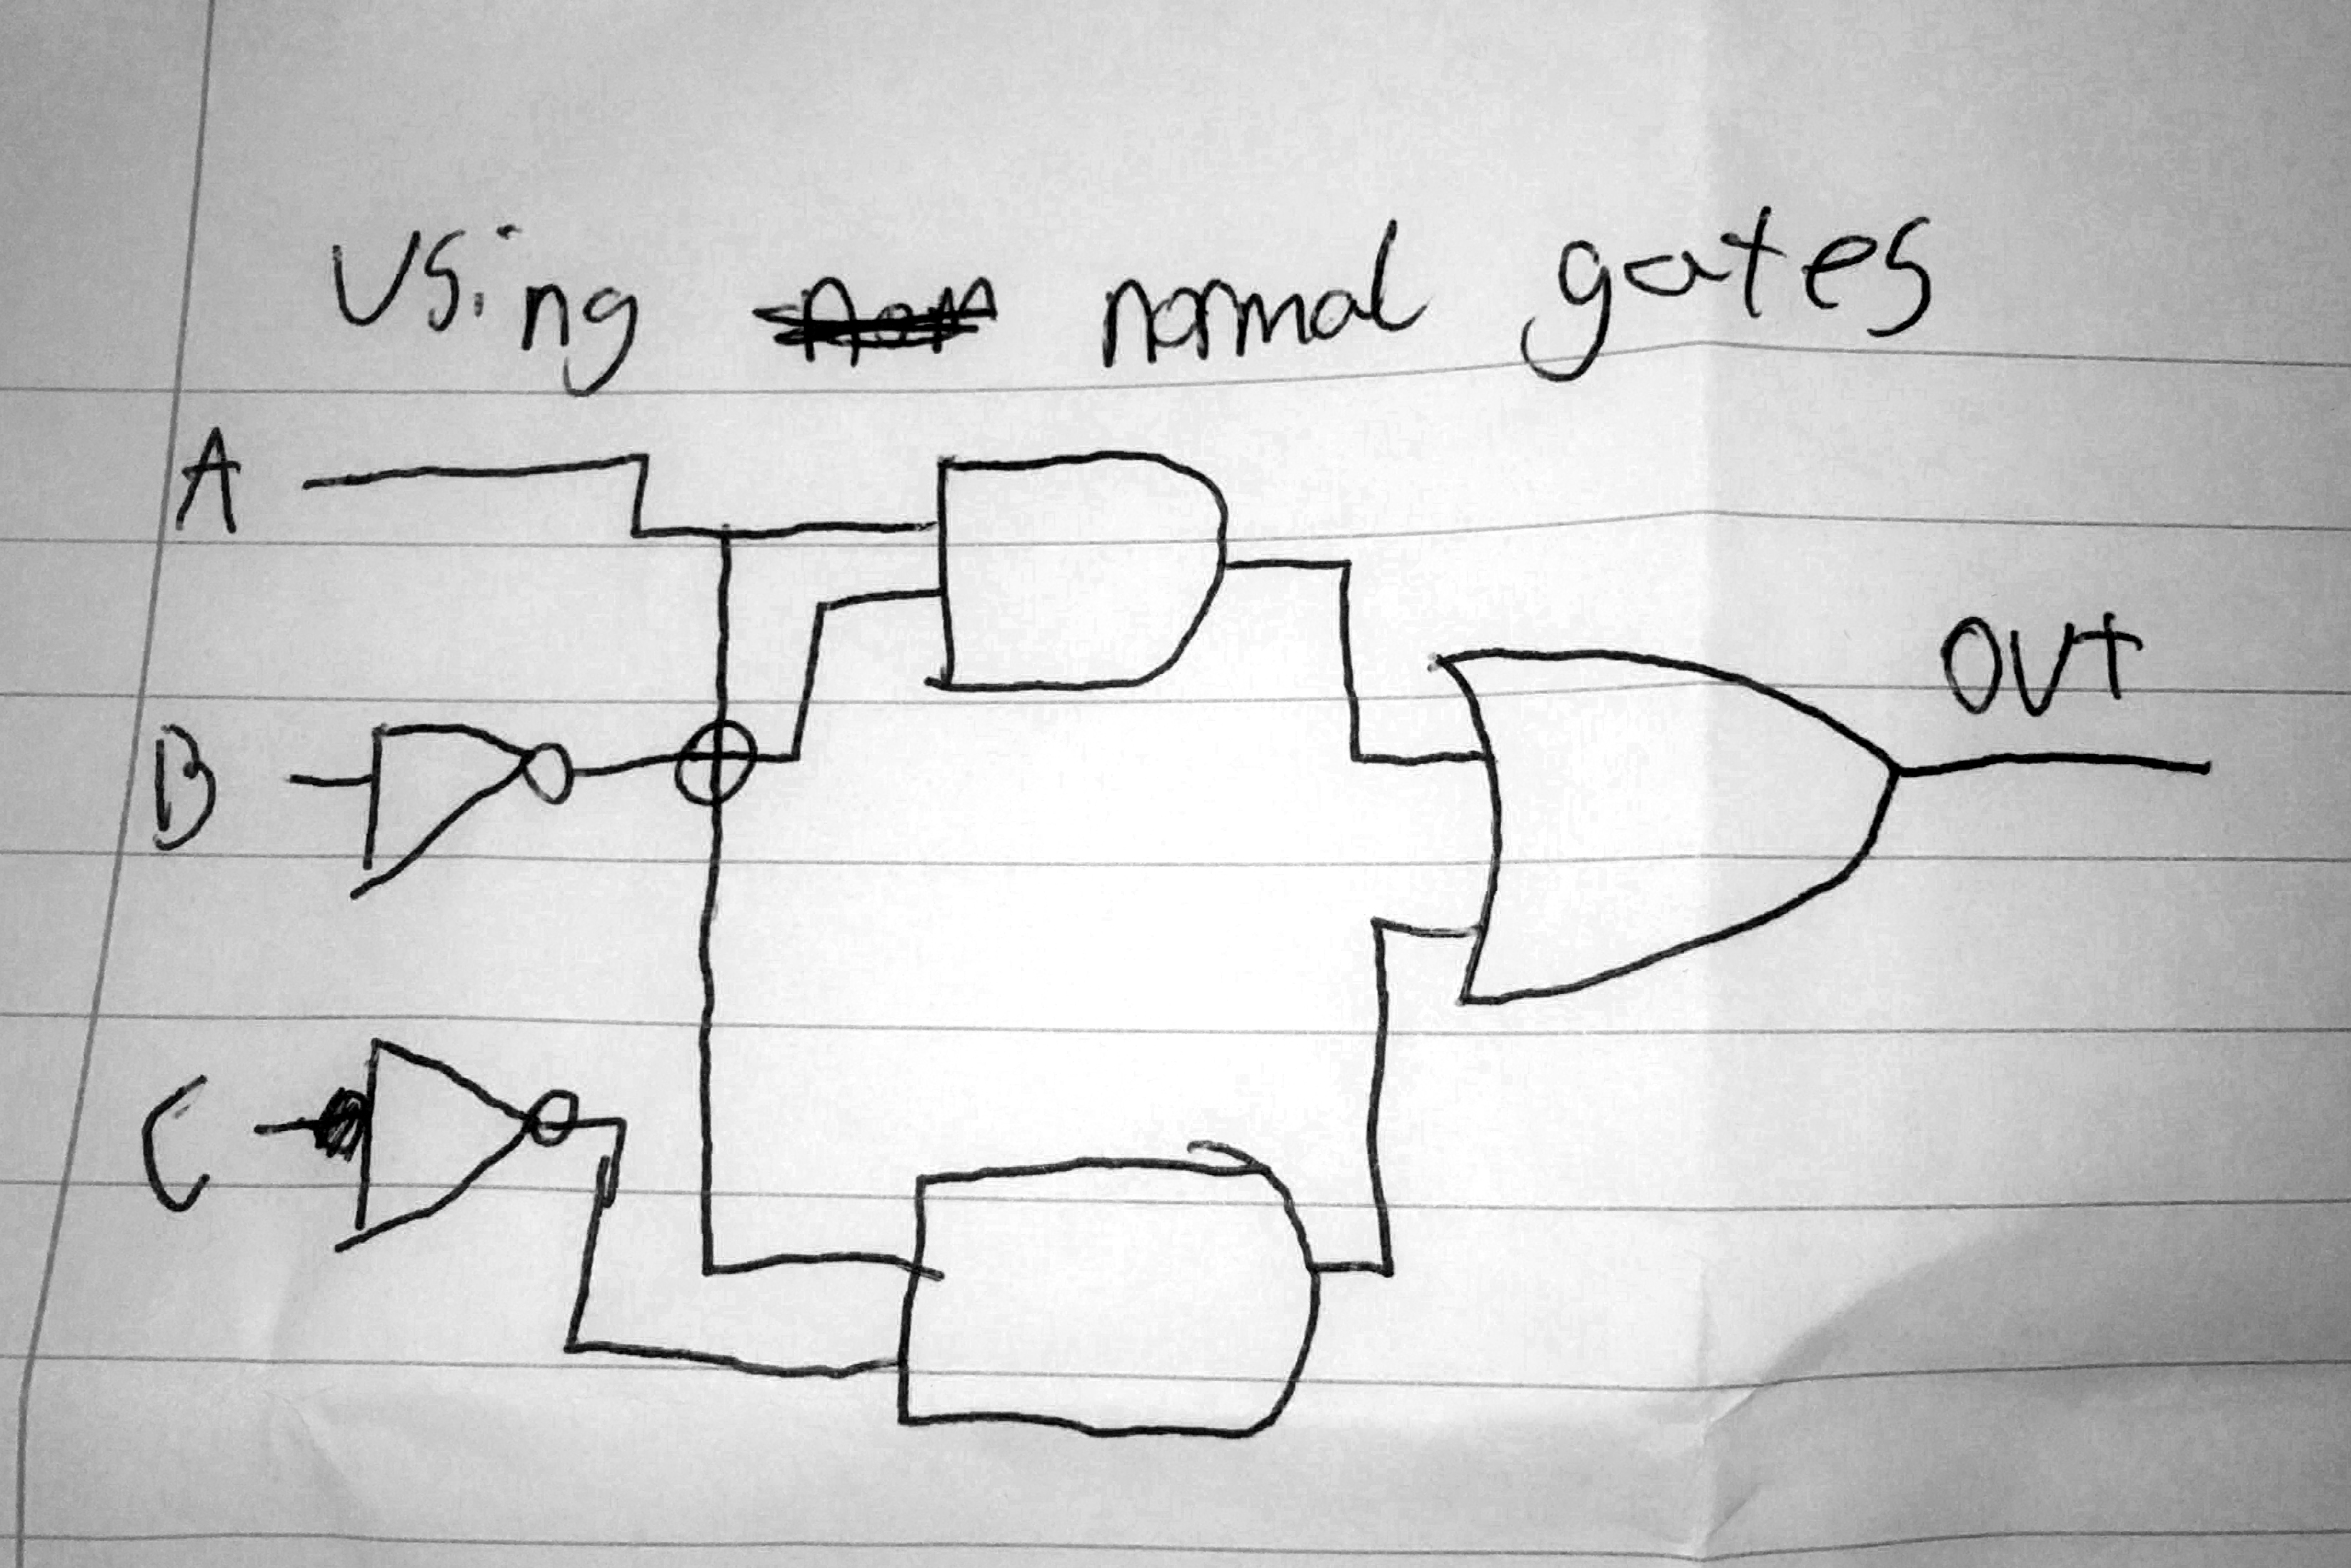
\includegraphics[width=\textwidth]{normal_gates.jpg}}

\subsection{Represent circuit using NAND gates}

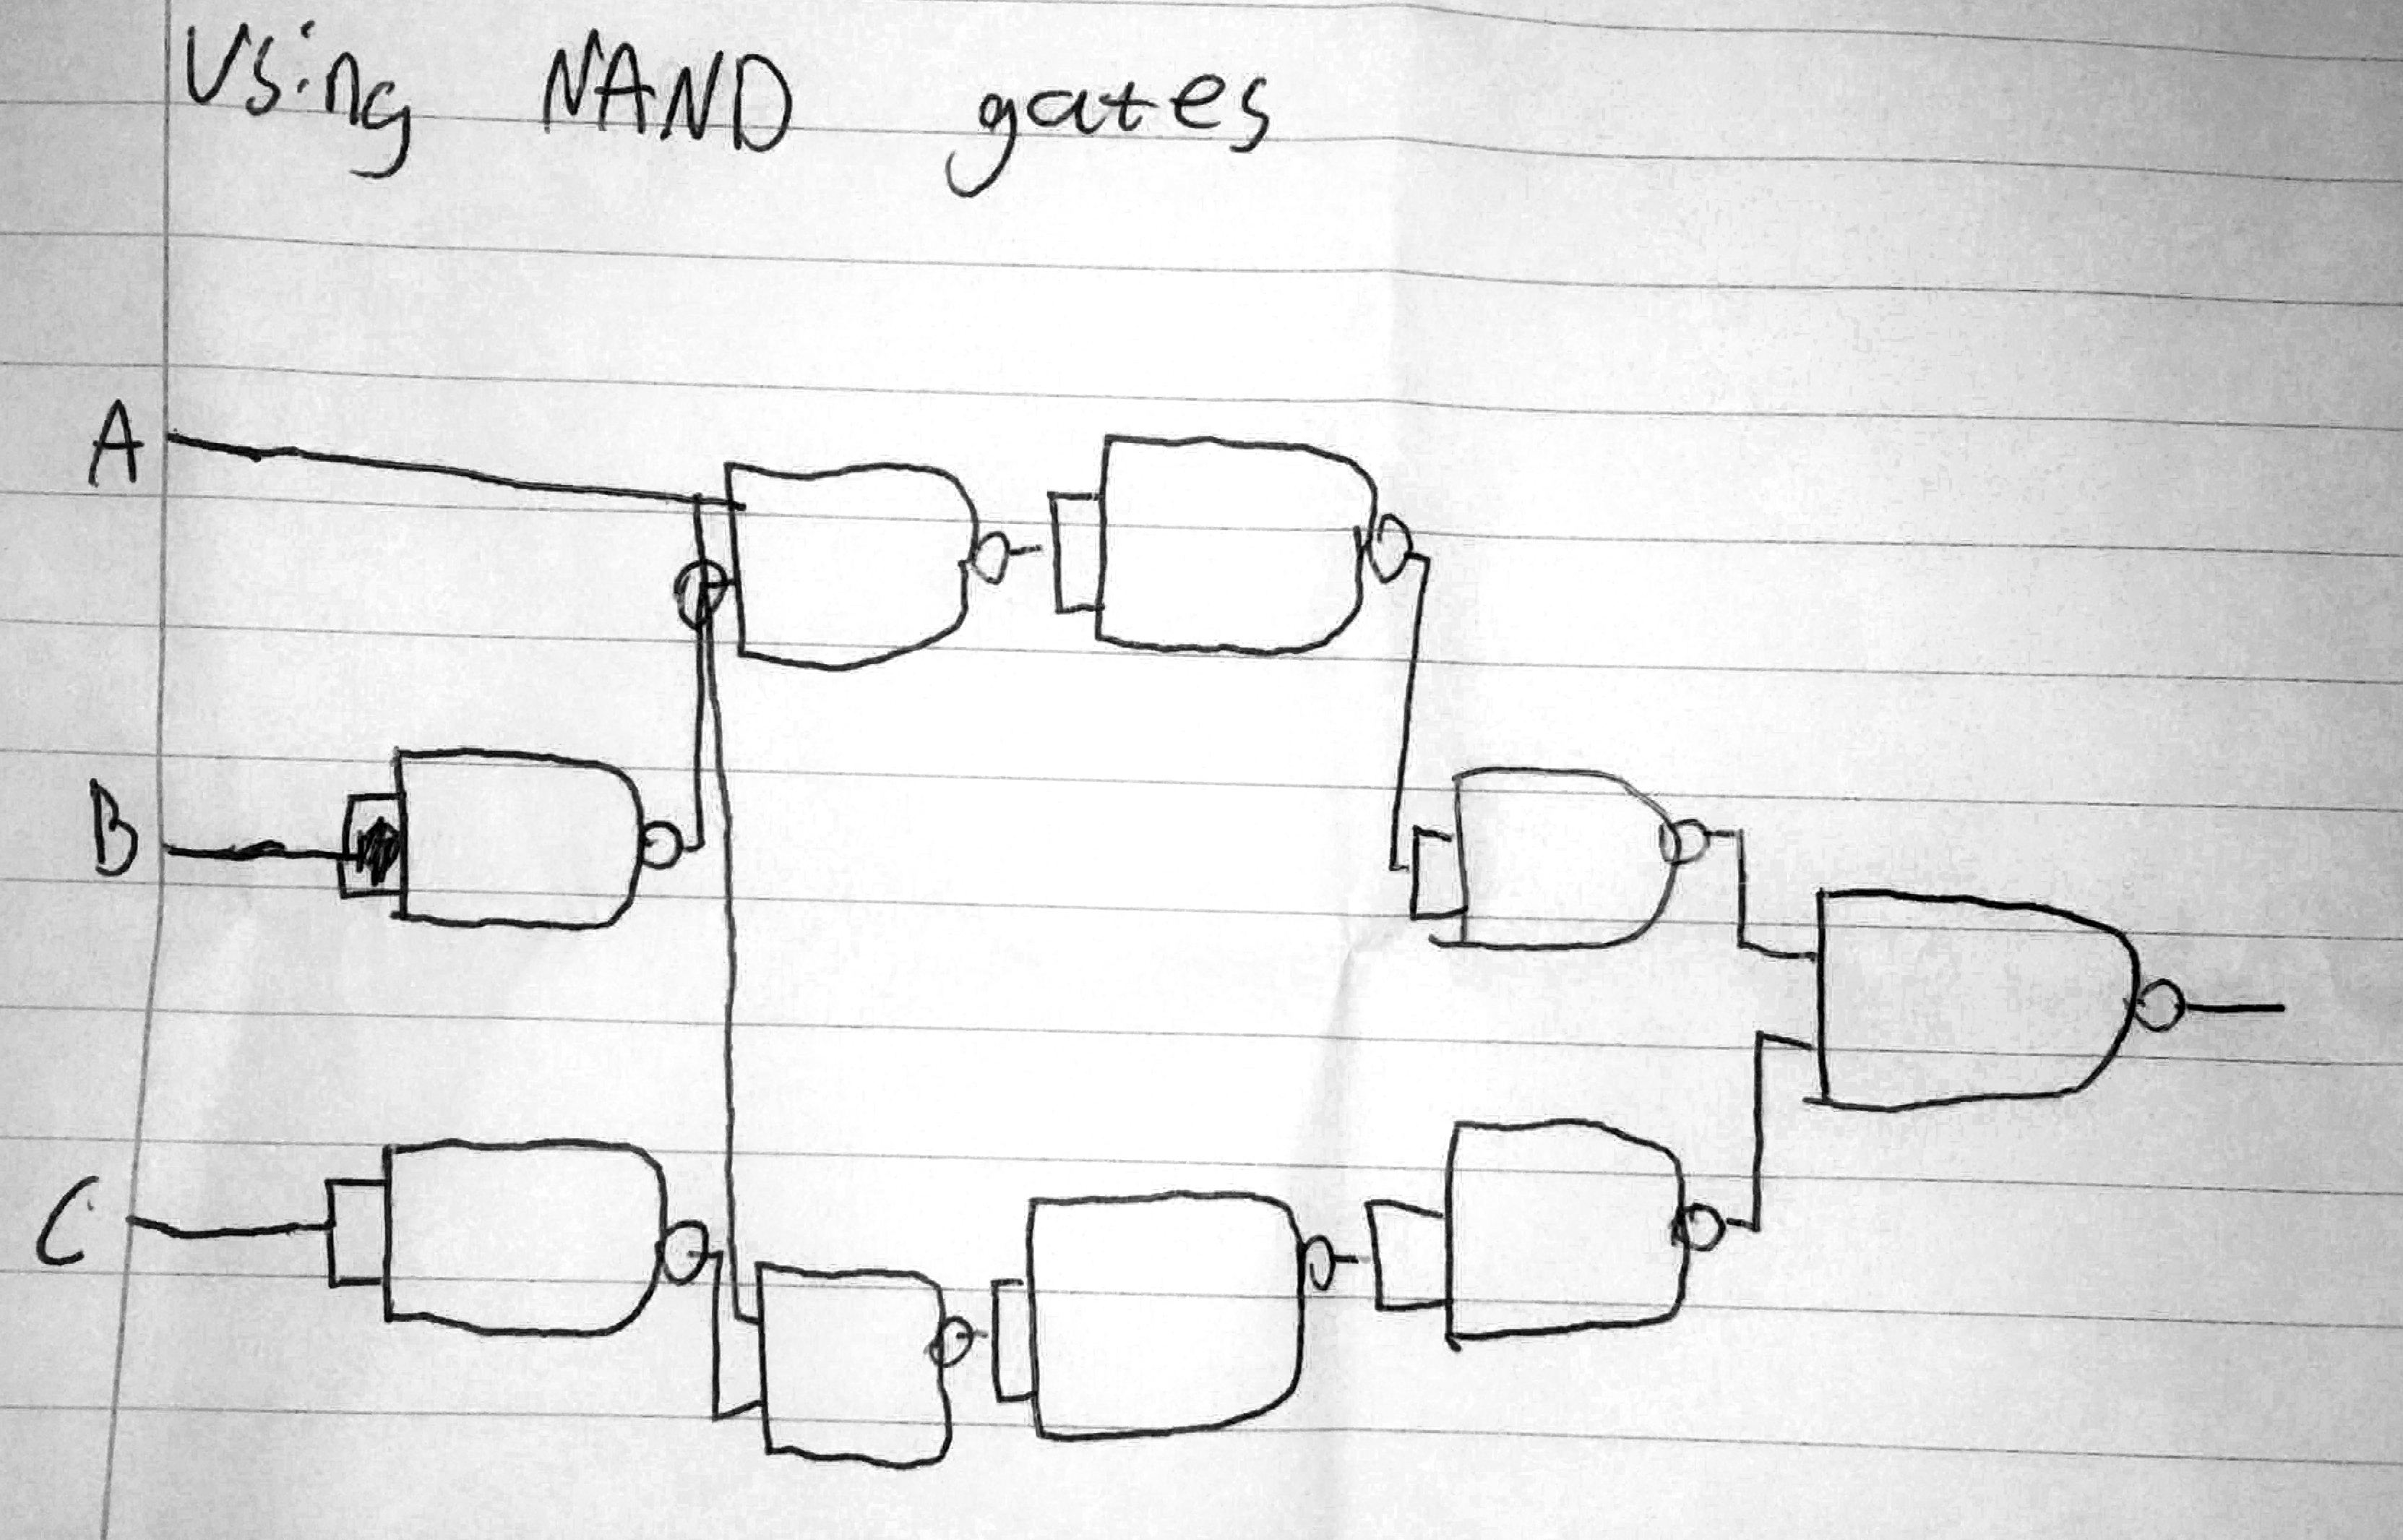
\includegraphics[width=\textwidth]{nand_gates.jpg}}

\section{Integration}

\subsection{$\int_{2}^{5} 2x^3$}

\[
\int_{2}^{5} 2x^3 = \left[\frac{x^4}{2} + C\right]_2^5
\]

\[
\left(\frac{5^4}{2} + C\right) - \left(\frac{2^4}{2} + C\right) = 312.5 - 8 = 304.5
\]

\subsection{$\int_{0}^{\frac{\pi}{2}} sin^2(x)$}

\[
\int_{0}^{\frac{\pi}{2}} sin^2(x) = \left[-\frac{\sin\left(2x\right)-2x}{4} +C\right]_0^{\frac{\pi}{2}}
\]

\[
\left(-\frac{\sin\left(2 \cdot \frac{\pi}{2}\right)-2 \cdot \frac{\pi}{2}}{4} +C\right) - \left(-\frac{\sin\left(2 \cdot 0\right)-2 \cdot 0}{4} +C\right) = \frac{\pi}{4} - \frac{-0}{4} = \frac{\pi}{4}
\]

\subsection{$\int 2x^2 \cdot ln(x)$}

\[2\left(\frac{x^3 \cdot ln(x)}{3} - \frac{x^3}{9}\right) +C\]

\[\frac{2x^3 (3\cdot ln(x) - 1)}{9} + C\]

\subsection{$ y= \int \frac{x^2}{2}sin(x)$ given that if $x=\pi$ then $y=1$}

??

\subsection{$\int e^x \cdot sin(x)$}

\[\frac{e^x(sin(x) - cos(x))}{2} + C\]

\section{Integration and design}

\subsection{Calculate the surface area of the front elevation of the bridge.}

Total surface area = $8 \cdot 20 = 160m^2$

Remove area of circles
\[160 - 4\pi = 147.43m^2\]

Remove area of the small boxes on either side
\[147.43 - 3 - 3 = 141.43m^2\]

Remove area of the big boxes on either side
\[141.43 - (4 \cdot 4) - (4 \cdot 4) = 109.43m^\]

Find estimated equation of arch
\[y=-0.375x^2 + 6\]

Integrate quation
\[6x-\frac{x^3}{8}\]

Find area under arch
\[32m^2\]

Remove area under arch
\[109.43 - 32 = 77.43m^2\]

The area of the front elevation of the bridge is $77.43m^2$.

\subsection{Calculate the volume and the mass of bricks required to
3 construct the railway bridge.}

The total volume of the bridge is $77.43 \cdot 6 = 464.58m^3$. The mass of the bridge would be $929,160kg$ tons. Or 929.16 tons.

\section{Further integration 1}

Since you no equation for the graph is given, it's difficult to integrate it to find the area under the graph. Instead I used a method of calculating the area of the shape of the bar formed by drawing the top from point to point. The shape this gives is a trapezoid.

To find the area of a trapezoid, the following equation can be used:
\[A = \frac{H_1 + H_2}{2} \cdot W\]

Since each data point had a spacing of one second, $W$ can be ignored. Thus to find the estimated distance flown in each second, I took the current velocity and added the next velocity and divided by 2. Then to find the total area, I summed up the result of all areas.

The rocket flew 64,818 meters during the rocket burn phase.

\section{Further integration 2}

\subsection{Average velocity between $A$ and $B$}

\[(0.013\cdot 70) + (\frac{0.0014 \cdot 20}{2}) + (\frac{0.0056 \cdot 20}{2}) = 0.91 + 0.014 + 0.056 = 0.98km\]

Between point A and B the car travelled 0.98km.

\[\frac{0.98}{0.013} = 75.38km/h\]

The driver travelled on average with a velocity of 75.38km/h between point A and B. Therefore he will not get a speeding ticket.

\subsection{Calculate average surface temperature}

No.

\section{Arithmetic and geometric series}

\subsection{For the series 1, 5, 9, 13 …, find the sum of the first 11 terms}

\[a=1, d=4\]

\[S_{11} = \frac{11}{2}(2+40)=231\]

\subsection{For the series -6, -6.8, -7.6 …, find the sum of terms 6 through to 10
inclusive.}

\[a=-6, d=-0.8\]

\[S_{6...10} = S_{10}-S_4\]

\[S_4=\frac{4}{2}(-12-2.4)=-28.8\]
\[S_{10}=\frac{10}{2}(-12-2.4)=-72\]

\[S_{6...10} = -42.2\]

\subsection{For the series 2, 4, 8, 16 … , find the 11
th term, and the sum of the first 13
terms.}

\[a=2, r=2\]
\[n_{11}=2\cdot2^{10}=2048\]
\[S_{13}=\frac{2(2^{13}-1)}{2-1}=16382\]

\subsection{For the series 3, -3.6, 4.32, -5.184… , find the 10
th term and state whether
this is a converging or a diverging series.}

\[a=3, r=-1.2\]
\[n_{10}=3\cdot-1.2^9=-15.48\]

The series is diverging.

\subsection{For the series -4, 3.2, -2.56, 2.048 … , find the 8
th term and the sum of an
infinite number of terms of this series.}

\[a=-4, r=-0.8\]
\[n_=-4\cdot-0.8^7=0.838\]
\[S_{\infty}=\frac{-4}{1--0.8}=2.\overline{2}\]

\section{Representing negative numbers in binary}

\subsection{Convert to two's complement binary 12-bit form}
\subsubsection{$-781$}
\[+781_2=001100001101\]

Invert it
\[110011110010\]

Add 1
\[-781_2=110011110011\]

\subsubsection{$-56$}
\[+56_2=000000111000\]

Invert it
\[111111000111\]

Add 1
\[-56_2=111111001000\]

\subsubsection{$-102$}
\[+102_2=000001100110\]

Invert it
\[111110011001\]

Add 1
\[-102_2=111110011010\]

\subsection{Perform the following calculations in binary}
\subsubsection{$78-671$}
\[78=000001001110\]
\[-671=110101100001\]
\[78+-671=110110101111\]

\subsubsection{$-376-78$}
\[-376=111010001000\]
\[-78=111110110010\]
\[-376+-78=111000111010\]

\section{Representing floating point numbers in binary}

\subsection{27.764}
\[27 = 11011\]
\[.764 = 1100001110010101100\]

Normalize
\[11011.1100001110010101100\]
\[1.10111100001110010101100\]
Moved 4 spaces to the left, thus exponent is 4.

The number is positive the sign bit is 0. When normalizing, the [dot] was moved 4 spaces to the left, so the exponent is 4. The biased exponent is 131. The mantissa is $10111100001110010101100$.

\begin{tabular}{l|l|l}
  Sign& Biased exponent & Mantissa \\
  \hline
  0& 10000011& 10111100001110010101100\\
\end{tabular}

\subsection{-416.2543}
\[416 = 110100000\]
\[.2543 = 010000010001101\]

Normalize
\[110100000.010000010001101\]
\[1.10100000010000010001101\]
Moved 8 spaces to the left, thus exponent is 8. Biased exponent is 135.


\begin{tabular}{l|l|l}
  Sign& Biased exponent & Mantissa \\
  \hline
  1 & 10000111 & 10100000010000010001101\\
\end{tabular}

\subsection{0.00476}
\[0 = 0\]
\[.00476 = 0000000100110111111100111000110\]

Normalize
\[0.0000000100110111111100111000110\]
\[000000001.00110111111100111000110\]
Moved 8 spaces to the right, thus exponent is -8. Biased exponent is 119.


\begin{tabular}{l|l|l}
  Sign& Biased exponent & Mantissa \\
  \hline
  0 & 01110111 & 00110111111100111000110\\
\end{tabular}

\section{Set theory}
Below are membership tables for each statement. If they are not equal the statement is false.

\subsection{$A \cap B = B \cap A$}

True.

\begin{table}[H]
\begin{tabular}{ll|ll}
A & B & $A⁡ \cap ⁡B$ & $B \cap ⁡A$ \\ \hline
0 & 0 & 0         & 0         \\
1 & 0 & 0         & 0         \\
0 & 1 & 0         & 0         \\
1 & 1 & 1         & 1        
\end{tabular}
\end{table}

\subsection{$\overline{A \cap B} = \overline{A} \cap \overline{B}$}

False.

\begin{table}[H]
\begin{tabular}{ll|ll}
A & B & $\overline{A \cap B}$ & $\overline{A} \cap \overline{B}$ \\ \hline
0 & 0 & 1         & 1         \\
1 & 0 & 1         & 0         \\
0 & 1 & 1         & 0         \\
1 & 1 & 0         & 0        
\end{tabular}
\end{table}

\subsection{$A \cap (B \cap C) = (A \cap B) \cap C$}

True.


\begin{table}[H]
\begin{tabular}{lll|ll}
A & B & C & $A \cap (B \cap C)$ & $(A \cap B) \cap C$ \\ \hline
0 & 0 & 0 & 0         & 0         \\
0 & 0 & 1 & 0         & 0         \\
0 & 1 & 0 & 0         & 0         \\
0 & 1 & 1 & 0         & 0         \\
1 & 0 & 0 & 0         & 0         \\
1 & 0 & 1 & 0         & 0         \\
1 & 1 & 0 & 0         & 0         \\
1 & 1 & 1 & 1         & 1         \\
\end{tabular}
\end{table}

\subsection{$A \cup (B \cap C) = (A \cup B) \cap C$}

False.

\begin{table}[H]
\begin{tabular}{lll|ll}
A & B & C & $A \cup (B \cap C)$ & $(A \cup B) \cap C$ \\ \hline
0 & 0 & 0 & 0         & 0         \\
0 & 0 & 1 & 0         & 0         \\
0 & 1 & 0 & 0         & 0         \\
0 & 1 & 1 & 1         & 1         \\
1 & 0 & 0 & 1         & 0         \\
1 & 0 & 1 & 1         & 1         \\
1 & 1 & 0 & 1         & 0         \\
1 & 1 & 1 & 1         & 1         \\
\end{tabular}
\end{table}

\subsection{$A \cup (B \cap C) = (A \cup B) \cap (A \cup C)$}

False.

\begin{table}[H]
\begin{tabular}{lll|ll}
A & B & C & $A \cup (B \cap C)$ & $(A \cup B) \cap C$ \\ \hline
0 & 0 & 0 & 0         & 0         \\
0 & 0 & 1 & 0         & 0         \\
0 & 1 & 0 & 0         & 0         \\
0 & 1 & 1 & 1         & 0         \\
1 & 0 & 0 & 1         & 0         \\
1 & 0 & 1 & 1         & 1         \\
1 & 1 & 0 & 1         & 1         \\
1 & 1 & 1 & 1         & 1         \\
\end{tabular}
\end{table}

\subsection{$\overline{B \setminus A} = \overline{A} \setminus \overline{B}$}

True.

\begin{table}[H]
\begin{tabular}{ll|ll}
A & B & $\overline{A \cap B}$ & $\overline{A} \cap \overline{B}$ \\ \hline
0 & 0 & 1         & 1         \\
1 & 0 & 0         & 0         \\
0 & 1 & 0         & 0         \\
1 & 1 & 1         & 1        
\end{tabular}
\end{table}

\subsection{$n(A) + n(B)$ and $n(A \cup B)$}

Always equal.

\subsection{$n(B) - n(a)$ and $n(B \setminus A)$}

Always equal.

\subsection{$n(A) \cdot n(B)$ and $n(A \cdot B)$}

Sometimes,...

\section{Discrete probability}

\subsection{Probability of life on K'Pac}

\[P(L=T, A=F) = 0.15 \cdot 0.9\]
\[P(L=T, A=T) = 0.75 \cdot 0.1\]

\[P(L=T)=0.9 \cdot 0.15 + 0.1 \cdot 0.75 = 0.21\]

There is a 21\% chance that there is some life form on K'Pax. Not bad but not good either.





\subsection{Given there is life, find probability of an oxygen atmosphere}

\[P(A|L) = \frac{P(L | A) \cdot P(A)}{P(L)}\]
\[P(A|L) = \frac{0.75 \cdot 0.1}{0.21} = 0.357\]

\end{document}
